\documentclass[a4paper, 12pt]{article}
\usepackage[margin=2cm]{geometry} 
\usepackage{amsmath,amsfonts}
\usepackage{amssymb,amsthm}
\usepackage{tikz,tkz-euclide}
\usepackage[cm]{fullpage}
\usepackage{fancyvrb}

\usetikzlibrary{calc,patterns,angles,quotes}
\usetkzobj{all}

\title{Senior Test 4}
\author{Stellenbosch Camp 2018}
\date{Time: $2 \frac{1}{2}$ hours}

\begin{document} \maketitle

\begin{enumerate}

\item[1.]  Prove that it is impossible to write a positive integer in every cell of an infinite chessboard, in such a manner that, for all positive integers $m, n$, the sum of numbers in every $m\times n$ rectangle is divisible by $m + n$.


\vspace{7pt}

% 
\item[2.] 

% Andrew geometry
% Asiatic Pacific Maths Olympiad, 1989, Q3
Let $A_1, A_2, A_3$ be three points in the plane, and for convenience, let $A_4 = A_1$, $A_5 = A_2$. For $n = 1, 2$ and $3$, suppose that $B_n$ is the midpoint of $A_n A_{n+1}$ and suppose that $C_n$ is the midpoint of $A_n B_n$. Suppose that $A_n C_{n+1}$ and $B_n A_{n+2}$ meet at $D_n$ and that $A_n B_{n+1}$ and $C_n A_{n+2}$ meet at $E_n$. Calculate the ratio of the area of triangle $\triangle D_1 D_2 D_3$ to the area of triangle $\triangle E_1 E_2 E_3$.

\vspace{5pt}

% (Iberoamerican Mathematical Olympiad shortlist 2009)
\item[3.]  

\vspace{7pt}

% 2017/2018 British MO Round 2
\item[4.]


\vspace{7pt}


\item[5.]   Let $p_1 = 2$ and define a sequence of prime numbers $p_1, p_2, p_3, \dots$ such that, for all positive integers $n$, $p_{n+1}$ is the least prime factor of $n \cdot p_1^{1!} \cdot p_2^{2!} \dots p_n^{n!} + 1$. Prove that all primes appear in the sequence.



\end{enumerate}

\vfill

%  Should be box and whiskers diagram here
\begin{figure}[h]
	\centering
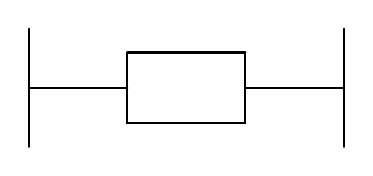
\begin{tikzpicture}[scale=0.25]
\tkzDefPoints{-8/3/o1, -8/-3/o2, 8/3/o3, 8/-3/o4, -3/1.8/o5, -3/-1.8/o6, 3/1.8/o7, 3/-1.8/o8,-3/0/w1, 3/0/w2, -8/0/w3, 8/0/w4}
\tkzDrawSegments[thick](o1,o2 o3,o4 o5,o6 o7,o8 o5,o7 o6,o8 w1,w3 w2,w4)

\end{tikzpicture}
\caption{This is \textbf{not} real math.}
\end{figure}

\vspace{12mm}

\end{document}
